\documentclass[letter]{beamer}
%removed: handout (ignores "animations")

\usepackage[utf8]{inputenc}
\usepackage{graphicx}
\usepackage{minted}

\usetheme{AnnArbor}
%\usetheme{CambridgeUS}
\usecolortheme{beaver}

\title[IIC2333] % (optional, only for long titles)
{07 - Capa de Red}
\subtitle{IIC2333 - Sistemas Operativos y Redes}
\author[C.Ruz] % (optional, for multiple authors)
{Cristian Ruz -- {\tt cruz@ing.puc.cl}\footnote{Material preparado con aporte del profesor Carlos Buil Aranda} }
\institute[PUC] % (optional)
{
  Departamento de Ciencia de la Computación\\
  Pontificia Universidad Católica de Chile
}
\date[2/2015] % (optional)
{Semestre 2-2015}
\subject{I}

\AtBeginSection[]
{
  \begin{frame}
    \frametitle{Contenidos}
    \tableofcontents[currentsection]
  \end{frame}
}

\begin{document}

%---------------------------------------------------------------------
\frame{\titlepage}


%---------------------------------------------------------------------
\begin{frame}
\frametitle{Contenidos}
%\tableofcontents[currentsection]
\tableofcontents
\end{frame}


%---------------------------------------------------------------------
\section{Modos de Conexión}

\begin{frame}
  \frametitle{Capa de Red}
  
  Objetivo: transmisión de unidades de datos desde un nodo emisor
  a un nodo receptor
  
  \begin{itemize}
    \item Unidad de datos: paquetes o datagramas
    \item Desafío: conseguir que los datagrams lleguen desde el nodo origen
          al nodo destino
    \item Arquitectura de enrutadores ({\em router}s)
    \item Algoritmos para determinar rutas (enrutamiento)
  \end{itemize}
  
\end{frame}
%---------------------------------------------------------------------
\begin{frame}
  \frametitle{Modos de Conexión}
  
  Establecer el camino de los datagramas es un problema antiguo

  \begin{center}
    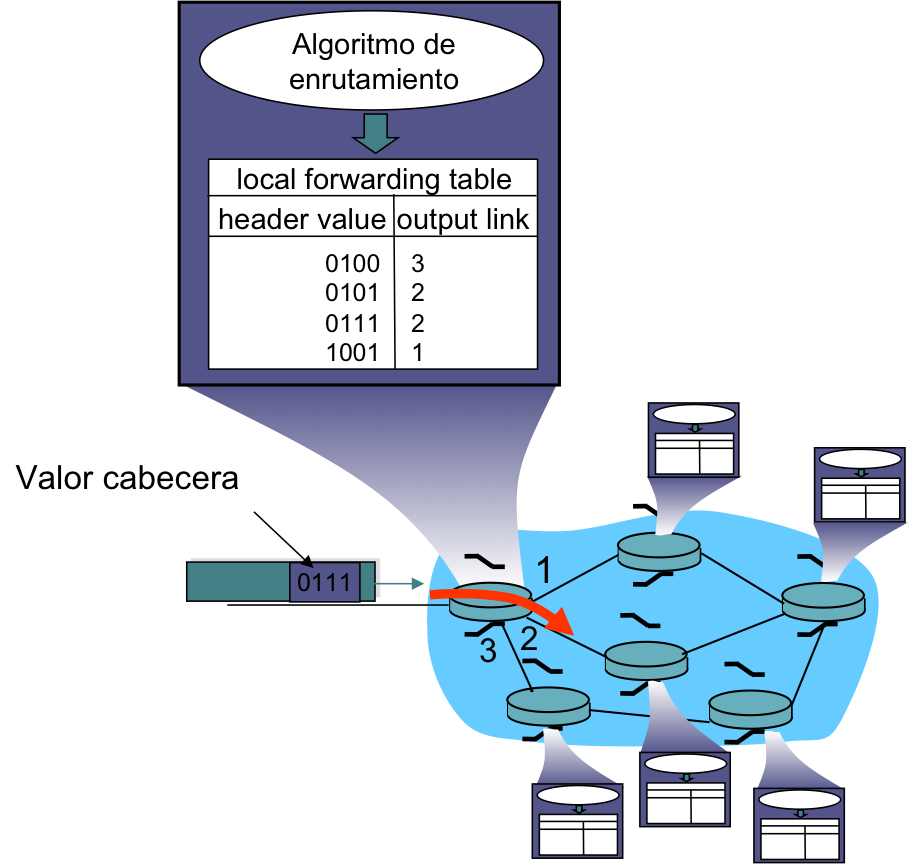
\includegraphics[width=5cm]{figs/07-redderouters.png}
  \end{center}
  
  Routers utilizando tablas para dirigir el tráfico entre distintas
  porciones de la red (subredes)

  Dos modelos de caminos: circuitos virtuales (orientado a conexión),
  y redes de datagramas (sin conexión)
\end{frame}

%---------------------------------------------------------------------
\begin{frame}
  \frametitle{Modos de Conexión}
  \framesubtitle{Circuitos Virtuales (CV)}
  
  \begin{itemize}
    \item Camino establecido antes de iniciar la transmisión
    \item Modelo de circuitos telefónicos
    \item Propiedades garantizables: ancho de banda, demora, QoS
    \item Paquetes usan número de circuito virtual en lugar de dirección de destino
    \item Estado de la conexión se mantiene a través de todos los {\em router}s
    \item Recursos dedicados
  \end{itemize}

\end{frame}
%---------------------------------------------------------------------
\begin{frame}
  \frametitle{Modos de Conexión}
  \framesubtitle{Circuitos Virtuales (CV)}

  \begin{center}
    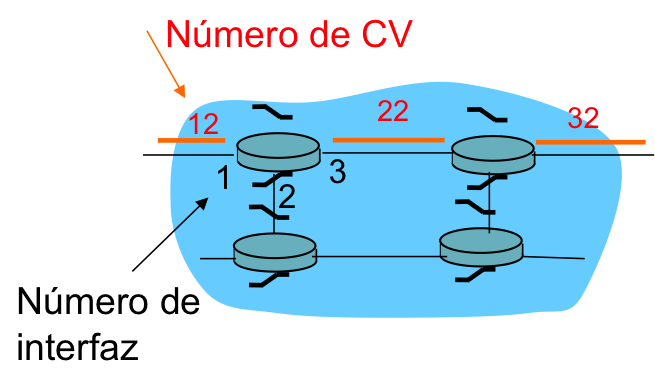
\includegraphics[width=5cm]{figs/07-cv.png}
  \end{center}

  \begin{center}
    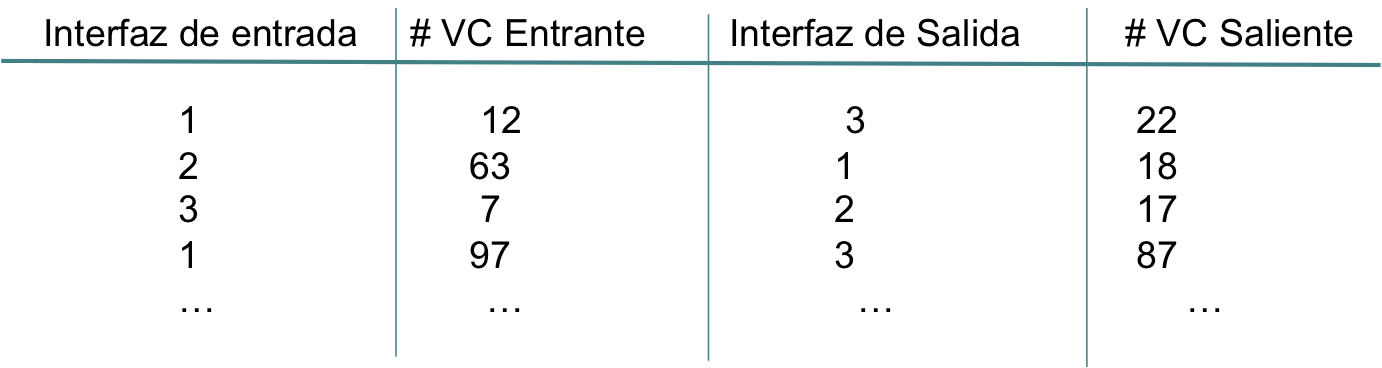
\includegraphics[width=10cm]{figs/07-cv-tabla.png}
  \end{center}

  Routers deben guardar estado de la conexión
  \begin{itemize}
    \item Protocolo de establecimiento de camino antes de transmitir
  \end{itemize}

\end{frame}
%---------------------------------------------------------------------
\begin{frame}
  \frametitle{Modos de Conexión}
  \framesubtitle{Redes de datagramas}

  No establece conexión
  \begin{itemize}
    \item Encabezados deben incluir dirección de destino
    \item Routers deciden ``libremente'' por dónde redirigir cada paquete
    \item Paquetes de entre mismo par $\langle$origen, destino $\rangle$ puede seguir
          distintos caminos
    \item Paquetes pueden llegar en orden distinto al que fueron enviados
  \end{itemize}
\end{frame}  
  
%---------------------------------------------------------------------
\begin{frame}
  \frametitle{Modos de Conexión}
  \framesubtitle{Redes de datagramas}

  Muchas direcciones de destino posibles
  \begin{itemize}
    \item Router utiliza rangos de direcciones
  \end{itemize}
  
  \begin{center}
    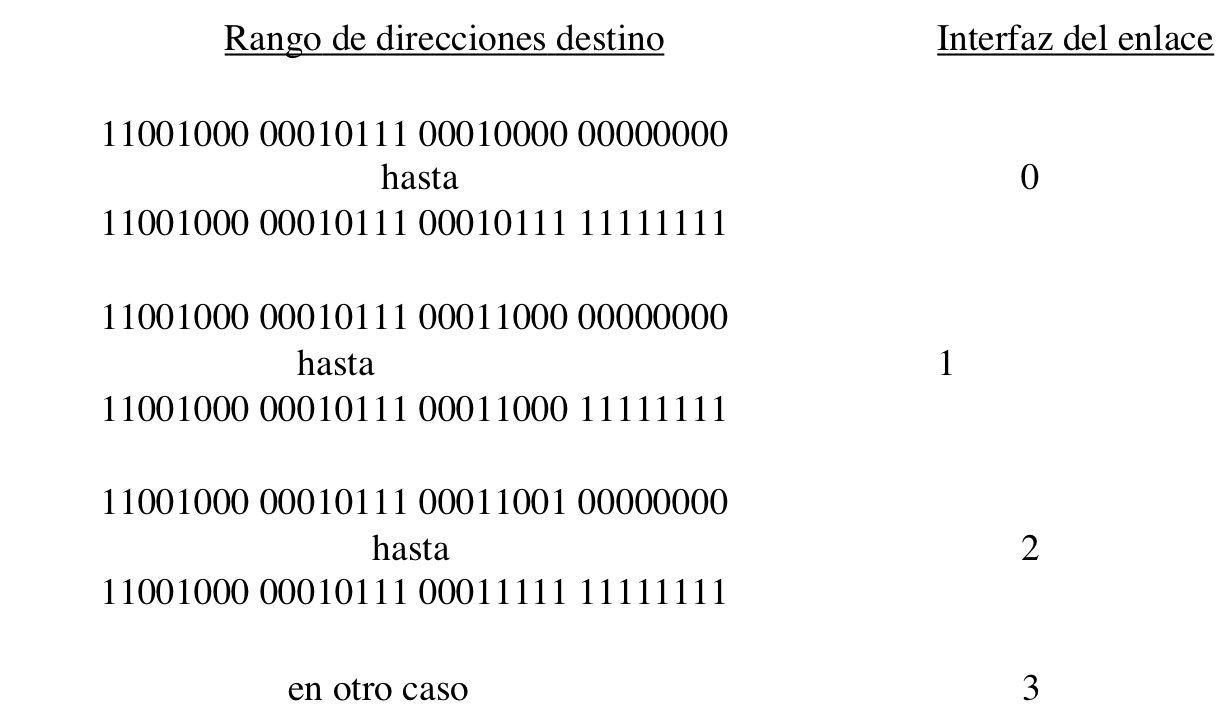
\includegraphics[width=10cm]{figs/07-datagrams-entries.png}
  \end{center}

\end{frame}

%---------------------------------------------------------------------
\begin{frame}
  \frametitle{Modos de Conexión}
  \framesubtitle{Circuitos Virtuales vs. Red de datagramas}

  Circuitos Virtuales
  \begin{itemize}
    \item Usando en servicio telefónico, redes ATM
    \item Calidad de servicio (QoS) garantizada
    \item Conexión no se establece si no se pueden garantizar recursos
    \item Sensible a congestiones
  \end{itemize}
  Redes de Datagramas
  \begin{itemize}
    \item Usado en Internet
    \item Servicio ``elástico'' sin garantías de tiempo
    \item Sistema flexible que puede adaptar control de flujo, velocidad de transmisión, usar múltiples rutas
    \item Difícil garantizar recursos durante la comunicación
  \end{itemize}

\end{frame}

%---------------------------------------------------------------------
\section{Direccionamiento IP y NAT}

\subsection{IP y Fragmentación}

\begin{frame}
  \frametitle{Header IP}

  IP: Internet Protocol
  \begin{center}
    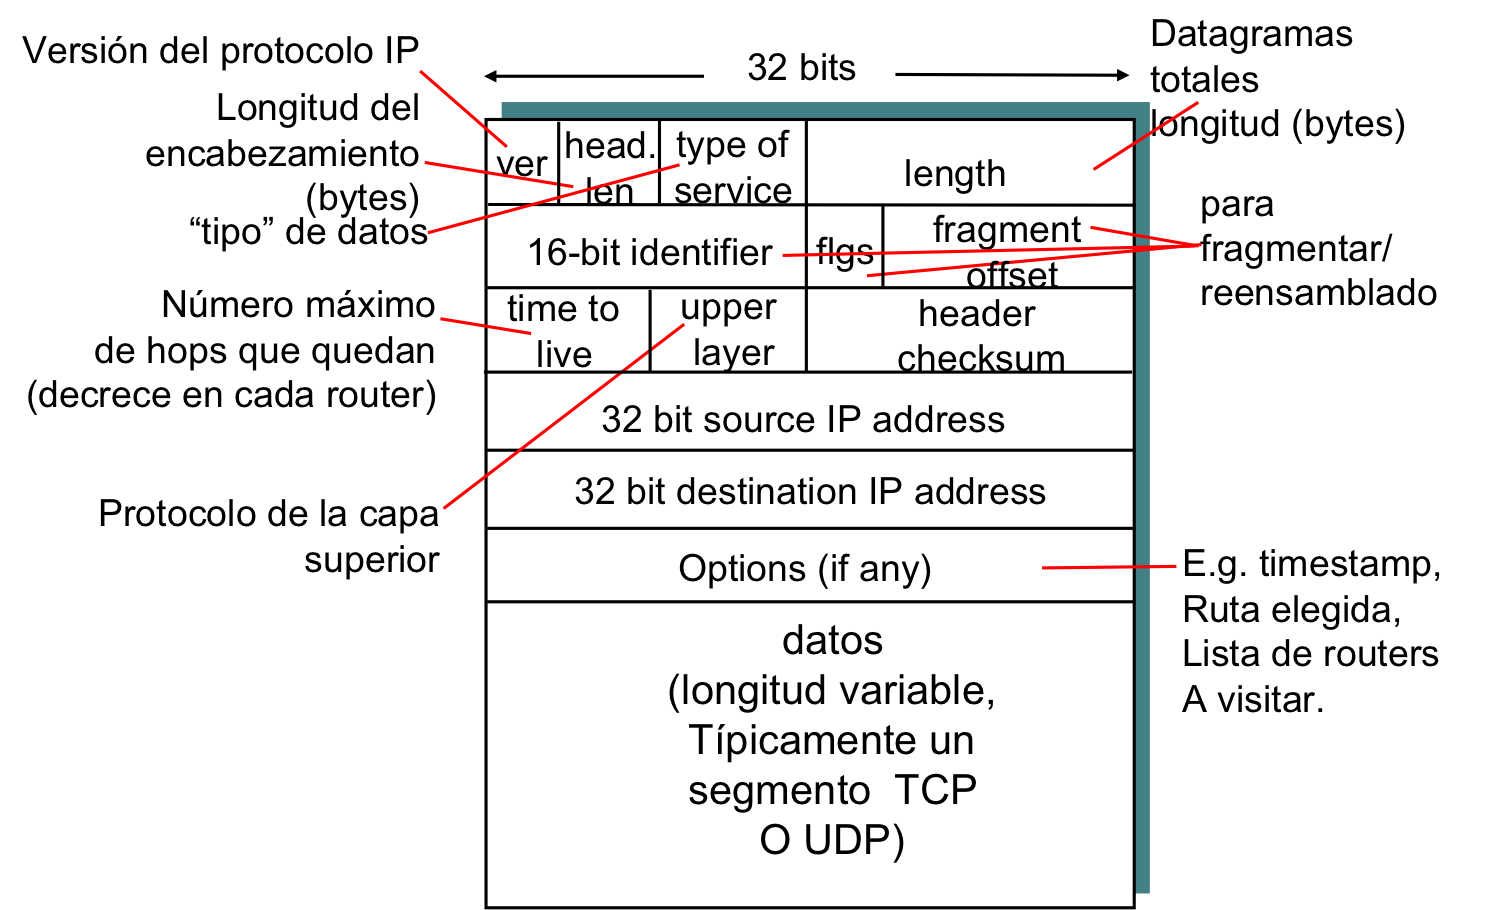
\includegraphics[width=10cm]{figs/07-ip-header.png}
  \end{center}
    
  
\end{frame}

%---------------------------------------------------------------------
\begin{frame}
  \frametitle{Fragmentación}

  Enlaces poseen una MTU: {\em Maximum Transfer Unit}.
  \begin{itemize}
    \item Tamaño máximo que puede ser transmitido en un enlace
    \item Paquetes pueden ser más grandes: son fragmentados y reensamblados
    \item Encabezado IP permite rearmarlos
  \end{itemize}

  \begin{center}
    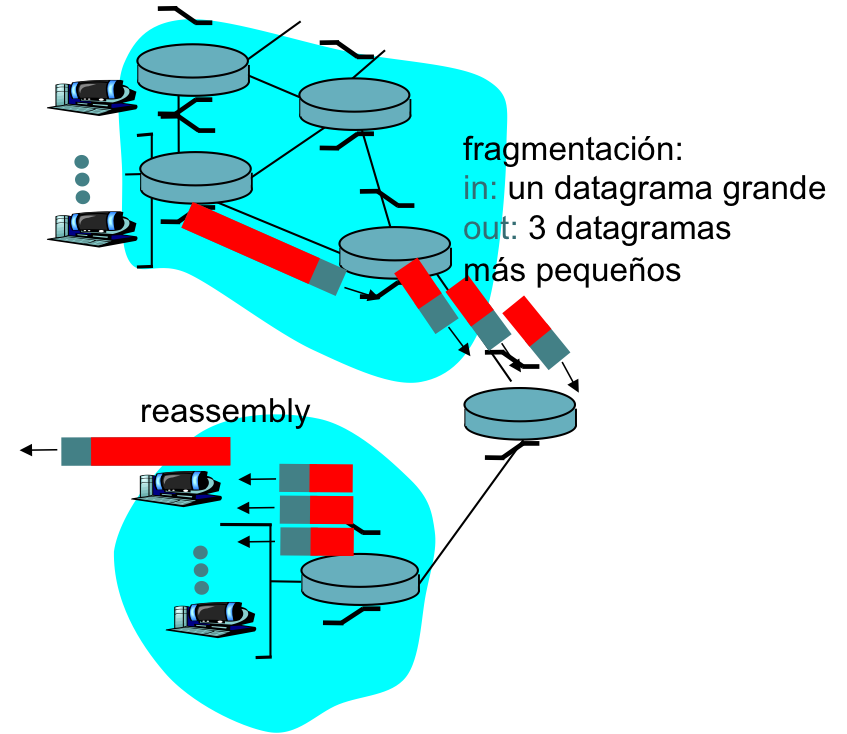
\includegraphics[width=6cm]{figs/07-ip-fragments.png}
  \end{center}

\end{frame}
%---------------------------------------------------------------------
\begin{frame}
  \frametitle{Fragmentación}

  \begin{center}
    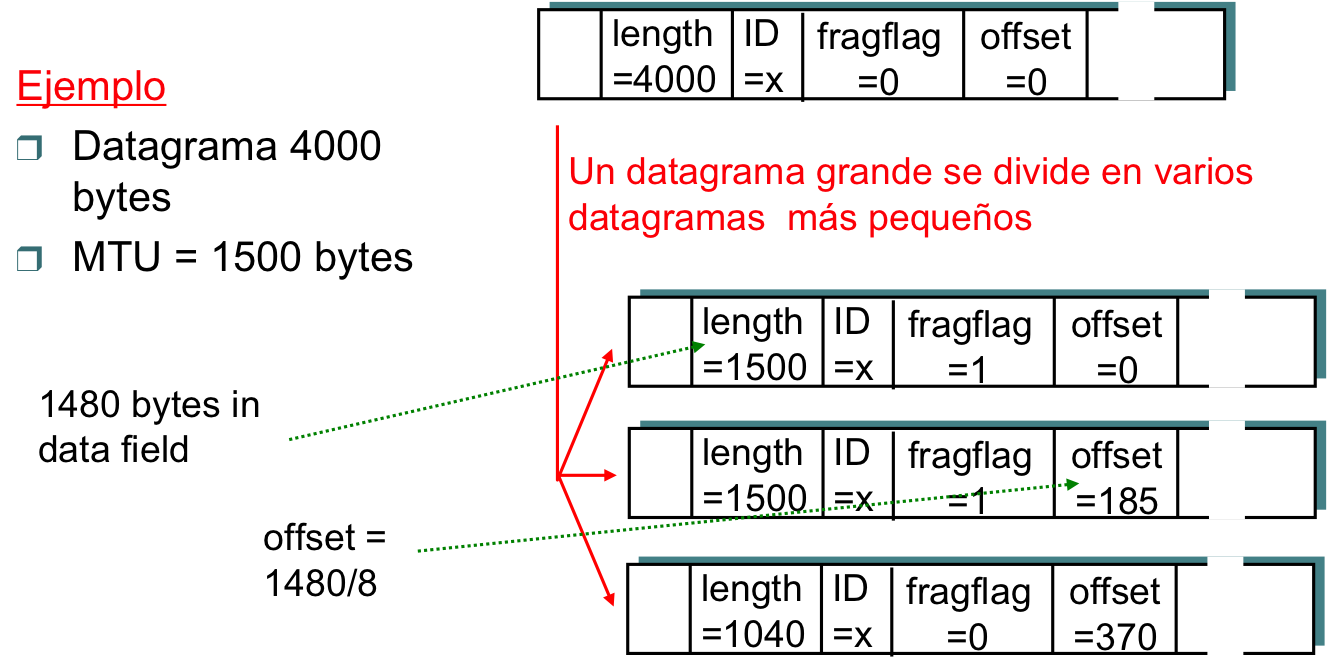
\includegraphics[width=10cm]{figs/07-ip-fragments-example.png}
  \end{center}

\end{frame}

%---------------------------------------------------------------------
\subsection{Direccionamiento IP}

\begin{frame}
  \frametitle{Direcciones IP}

  Identificador de 32-bit (IPv4) en notación {\em dotted-decimal}
  
  \begin{itemize}
    \item Identificador para interfaces (de host o de router)
    \item {\em Router} suele tener múltiples interfaces
    \item {\em Host} suelen tener sólo uan interfaz
    \item Dirección IP está asociada a una interfaz
  \end{itemize}

  \begin{center}
    146.155.13.45 = 10010010.10011011.00001101.00101101
  \end{center}  
  
\end{frame}
%---------------------------------------------------------------------
\begin{frame}
  \frametitle{Direcciones IP y Subredes}

  Una {\bf subred} se define por un grupo de los bits más altos de una dirección IP
  \begin{itemize}
    \item Bits más altos definen la subred
    \item Bits más bajos definen el {\em host}
  \end{itemize}
  
  Miembros de una misma subred pueden alcanzar sin necesitar un {\em router}
  
  \begin{center}
    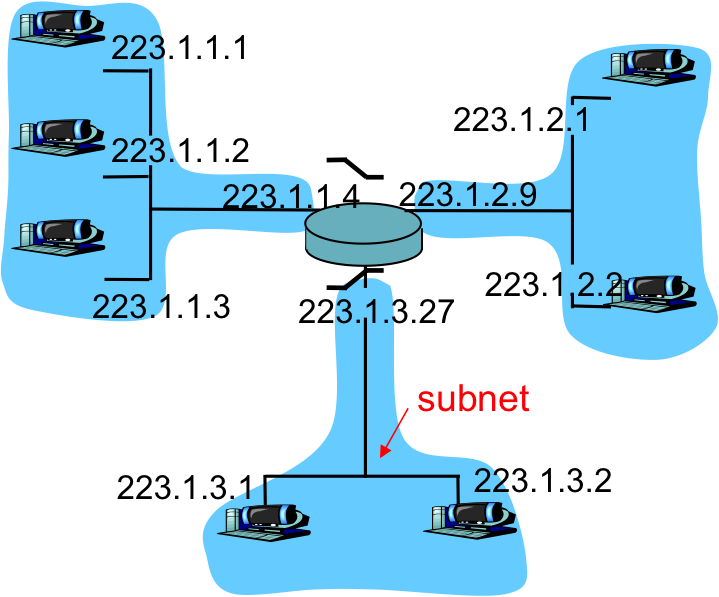
\includegraphics[width=6cm]{figs/07-ip-subnets.png}
  \end{center}
  
\end{frame}
%---------------------------------------------------------------------
\begin{frame}
  \frametitle{Direcciones IP y Subredes}
  \framesubtitle{Subredes especiales}
  
  \begin{itemize}
    \item 0.0.0.0. Dirección del host actual (sólo sirve como origen)
    \item 127.0.0.0. Dirección {\em loopback}
    \item Sección de {\em host}=0. Dirección de la subred
    \item Sección de {\em host}=1. Dirección {\em broadcast} de la subred
  \end{itemize}

\end{frame}
%---------------------------------------------------------------------
\begin{frame}
  \frametitle{Direcciones IP y Subredes}
  \framesubtitle{CIDR: Classless InterDomain Routing}


  \begin{center}
    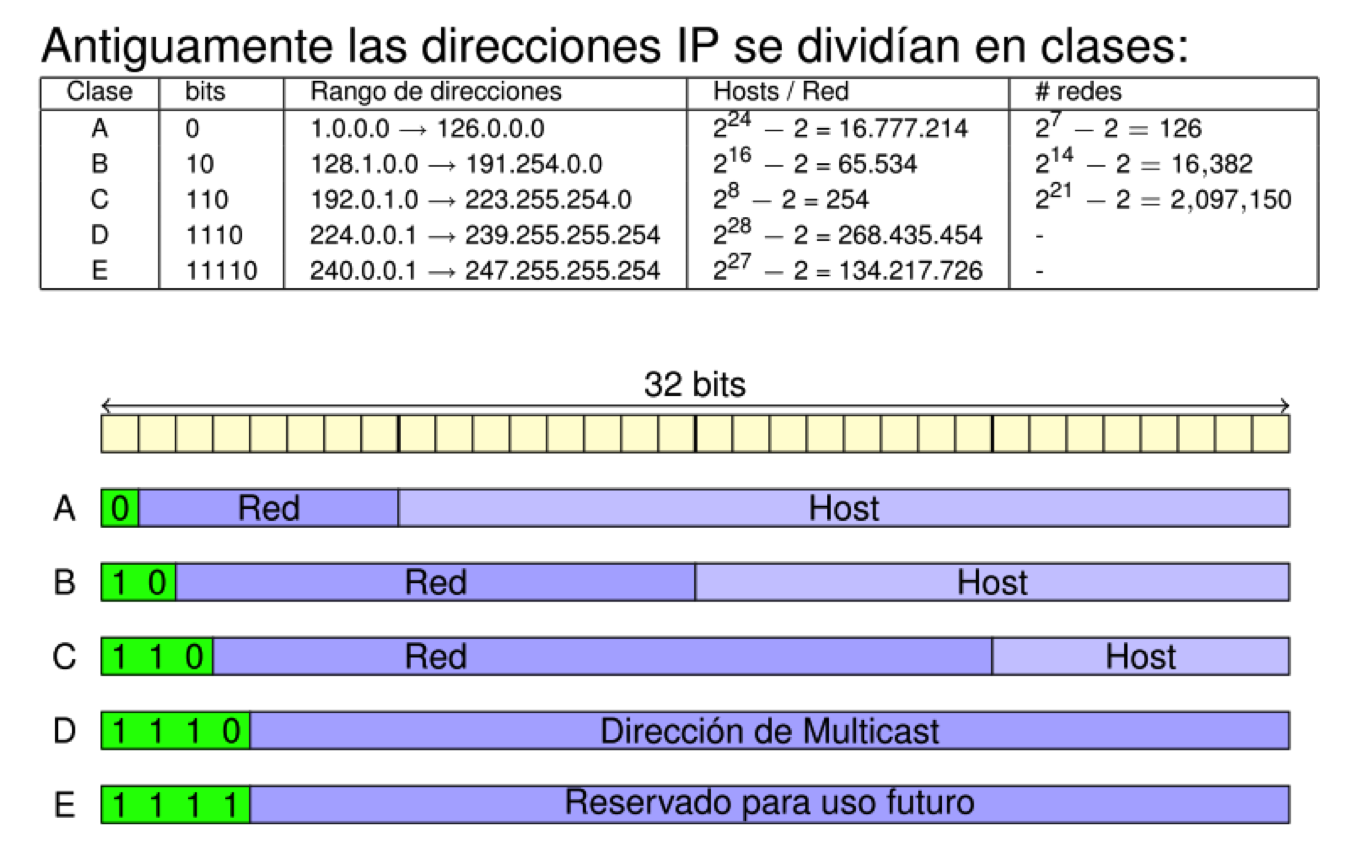
\includegraphics[width=10cm]{figs/07-ip-subnets-clases.png}
  \end{center}

\end{frame}

%---------------------------------------------------------------------
\begin{frame}
  \frametitle{Direcciones IP y Subredes}
  \framesubtitle{CIDR: Classless InterDomain Routing}

  Permite definir arbitrariamente porción de subred y de host
  \begin{itemize}
    \item Formato: {\tt a.b.c.d/x}, donde {\tt x} es la cantidad de bits de la subred.
    \item Ejemplo: 146.155.13.0/24 indica la subred en que todas las direcciones empiezan con 146.155.13
  \end{itemize}

  \begin{center}
    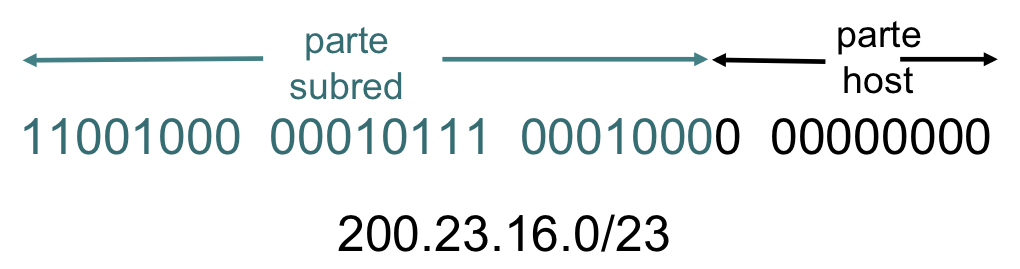
\includegraphics[width=10cm]{figs/07-ip-subnets-cidr.png}
  \end{center}
  
\end{frame}
%---------------------------------------------------------------------
\begin{frame}
  \frametitle{Direcciones IP y Subredes}
  \framesubtitle{Subredes especiales}

  \begin{itemize}
    \item Red local: 0.0.0.0/8
    \item Red loopback: 127.0.0.0/8
    \item Redes privadas: 10.0.0.0/8, 172.16.0.0/12, 192.168.0.0/16
  \end{itemize}

  La cantidad de bits disponibles para el {\em host} determina la cantidad de {\em hosts} posible
    
\end{frame}

%---------------------------------------------------------------------
\begin{frame}
  \frametitle{Direcciones IP y Subredes}

  \begin{center}
    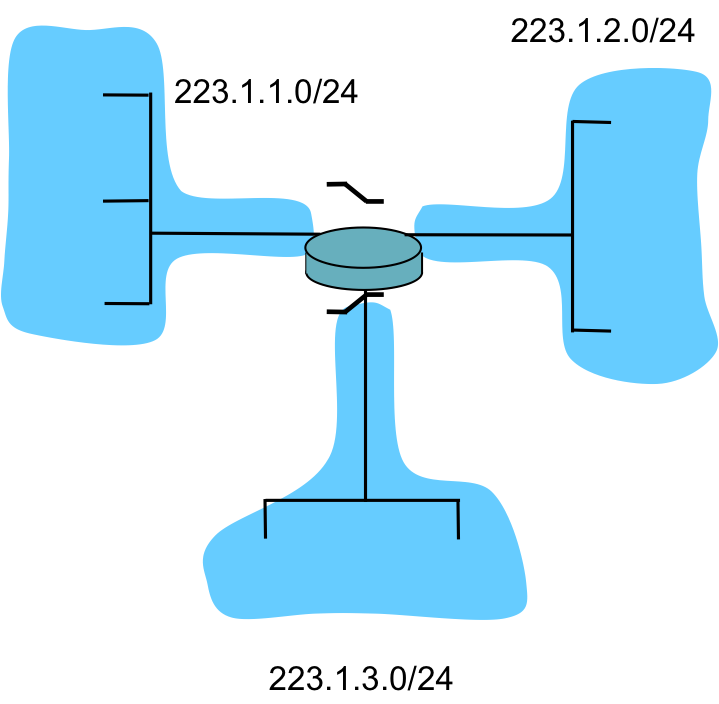
\includegraphics[width=7cm]{figs/07-ip-subnets-2.png}
  \end{center}
  

\end{frame}
%---------------------------------------------------------------------
\begin{frame}
  \frametitle{Direcciones IP y Subredes}

  \begin{center}
    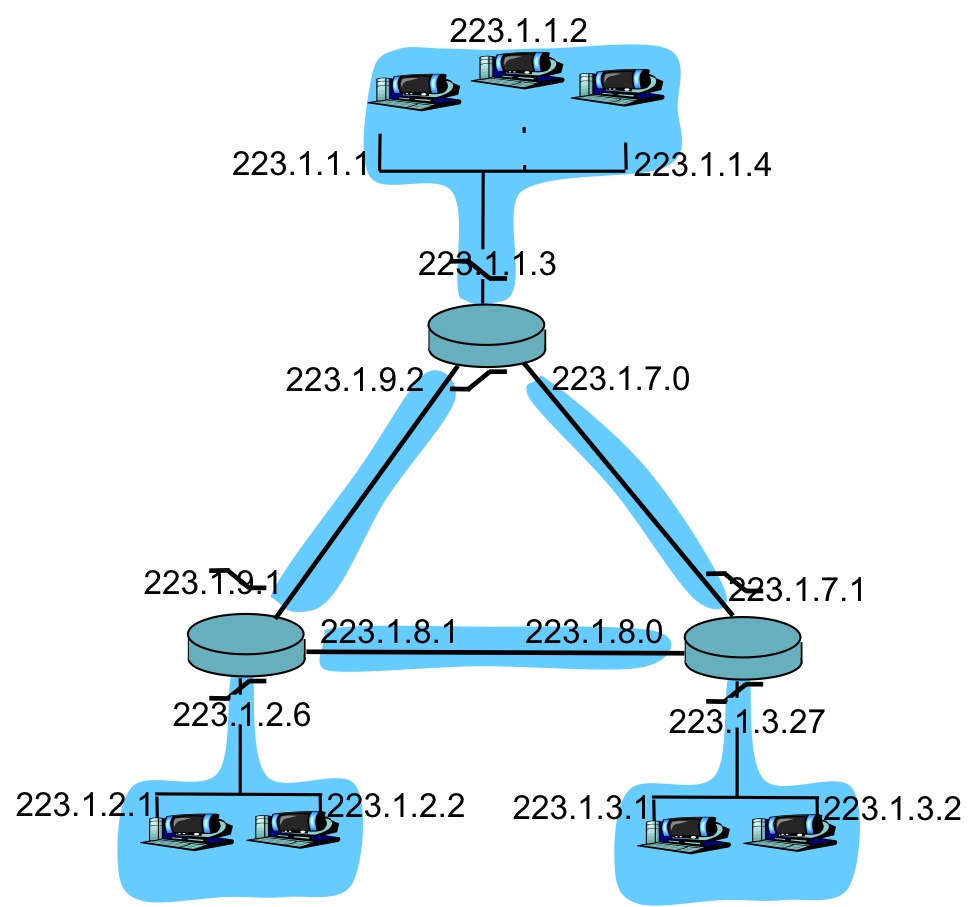
\includegraphics[width=7cm]{figs/07-ip-subnets-3.png}
  \end{center}
  

\end{frame}

%---------------------------------------------------------------------
\begin{frame}
  \frametitle{DHCP}
  \framesubtitle{Dynamic Host Configuration Protocol}
  
  ¿Como obtener una dirección?
  \begin{itemize}
    \item Manualmente
    \item Ó vía DHCP
  \end{itemize}
  
  DHCP permite asignar direcciones IP dinámicamente dentro de una subred
  \begin{itemize}
    \item Host envía mensaje broadcast: DHCP DISCOVER
    \item DHCP responde con mensaje: DHCP OFFER
    \item Host solicita dirección IP: DHCP REQUEST
    \item DHCP confirma solicitud: DHCP ACK
  \end{itemize}

\end{frame}
%---------------------------------------------------------------------
\begin{frame}
  \frametitle{DHCP}
  \framesubtitle{Dynamic Host Configuration Protocol}

  \begin{center}
    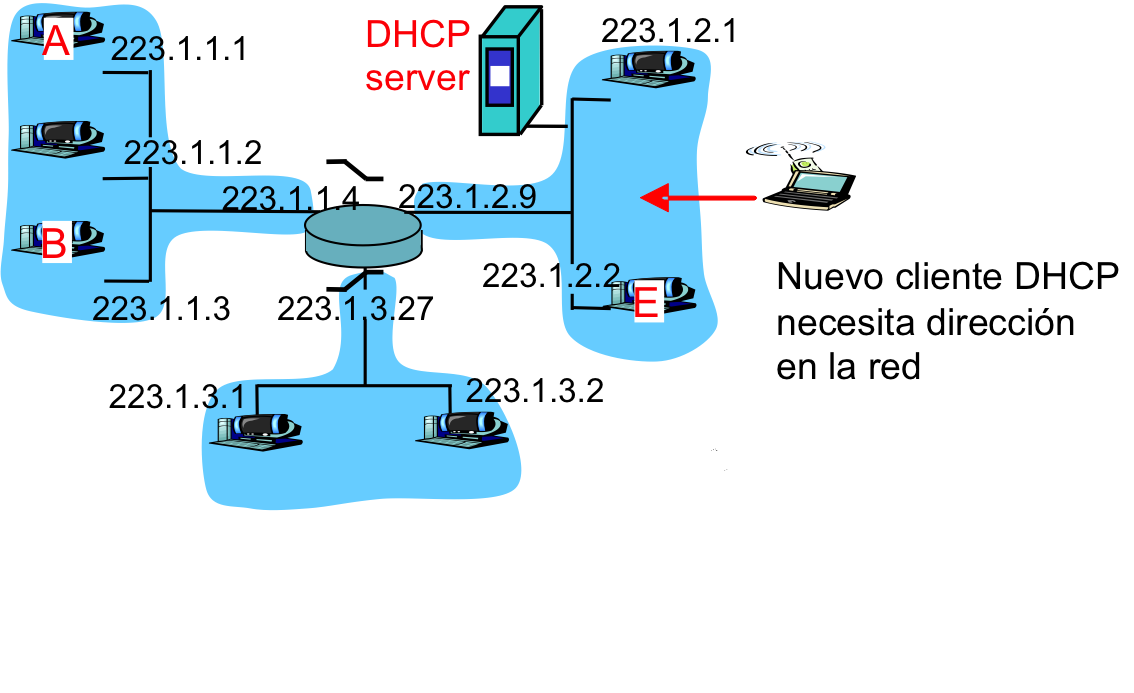
\includegraphics[width=10cm]{figs/07-dhcp.png}
  \end{center}

\end{frame}
%---------------------------------------------------------------------
\begin{frame}
  \frametitle{DHCP}
  \framesubtitle{Dynamic Host Configuration Protocol}

  \begin{center}
    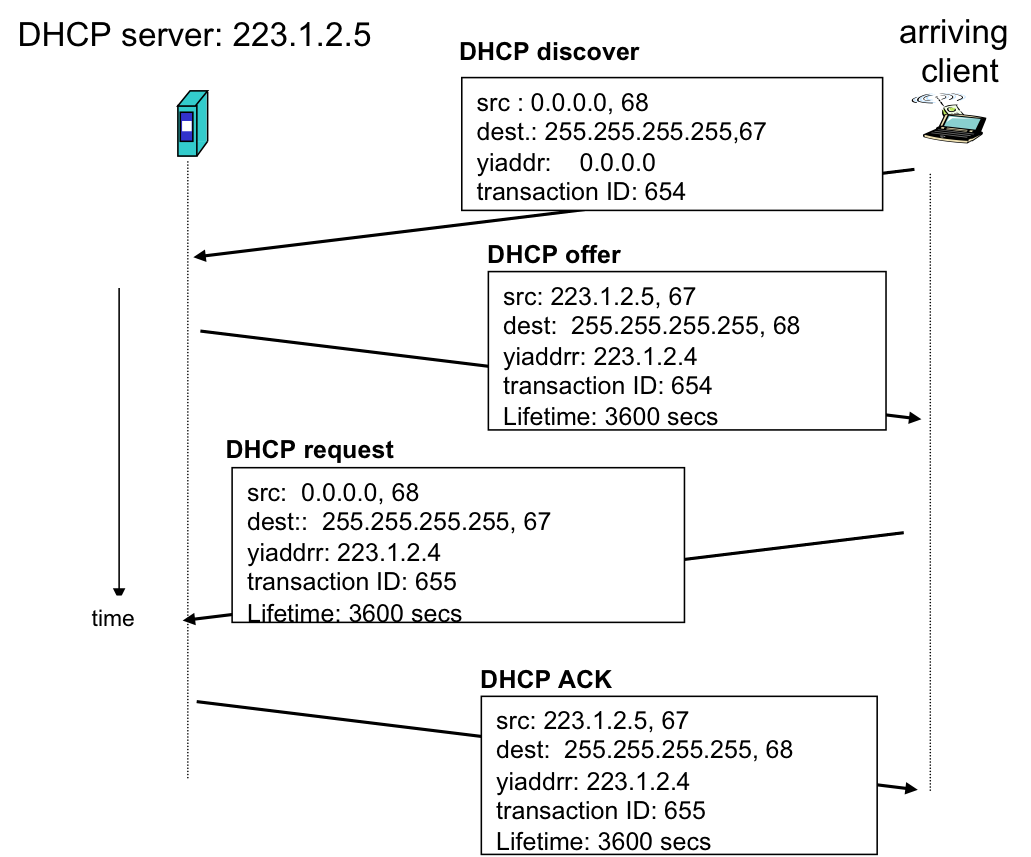
\includegraphics[width=8cm]{figs/07-dhcp-2.png}
  \end{center}

\end{frame}
%---------------------------------------------------------------------
\begin{frame}
  \frametitle{¿Cómo obtener direcciones IP}

  ISP obtienen rangos de direcciones IP a través de ICANN
  \begin{itemize}
    \item ICANN: Internet Corporation for Assigned Names and Numbers
    \begin{itemize}
      \item Asigna rangos de direcciones
      \item Gestiona DNS
      \item Asigna puertos y servicios estándar
    \end{itemize}
  \end{itemize}
\end{frame}

%---------------------------------------------------------------------
\begin{frame}
  \frametitle{¿Qué hacer con el término de las direcciones IP?}

  Direcciones IPv4 tienen 32-bit: $2^{32}$ direcciones posibles, $\sim 4.3 \times 10^9$
  \begin{itemize}
    \item Último rango top-level asignado en Febrero 2011
    \item Desde entonces se han recuperado rangos de direcciones
  \end{itemize}
  Solución definitiva: migrar a IPv6
  \begin{itemize}
    \item Direcciones de 128-bit: $2^{128}$ direcciones (es ¡mucho!)
    \item Notación: 8 grupos de 4 dígitos hexadecimales
    \item Ejemplo: 2001:0db8:85a3:0042:1000:8a2e:0370:7334
    \item Hasta Mayo 2014, el 96\% del tráfico usa IPv4
  \end{itemize}

\end{frame}
%---------------------------------------------------------------------
\subsection{NAT}

\begin{frame}
  \frametitle{NAT}
  \framesubtitle{Network Address Translation}

  ¿Como comunicarse con nodos en un red privada (interna)?

  \begin{center}
    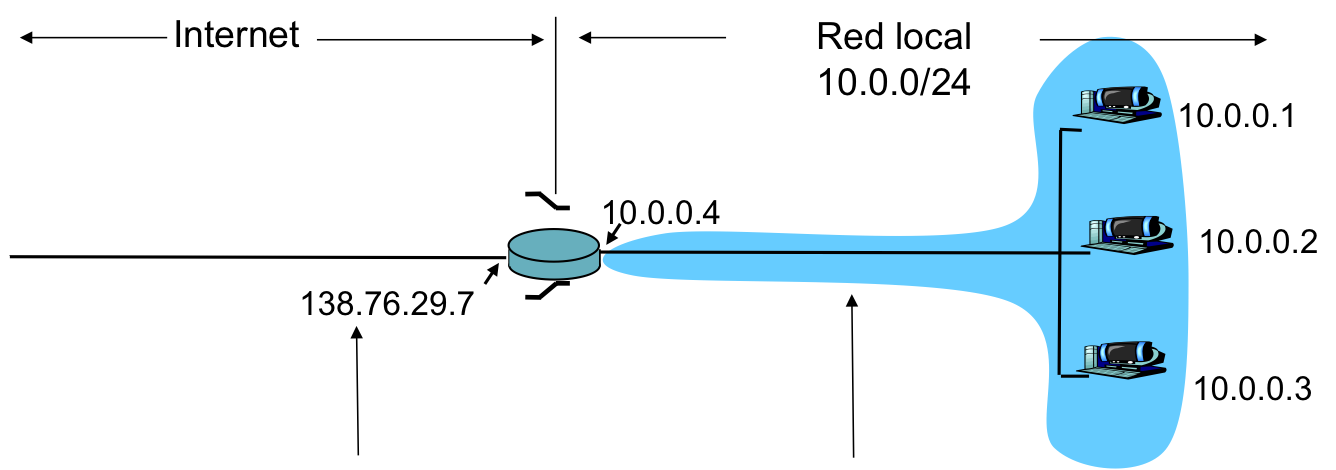
\includegraphics[width=10cm]{figs/07-nat-1.png}
  \end{center}

  \begin{itemize}
    \item Paquetes en la red interna tiene dirección de origen en 10.0.0.0/24
    \item Paquetes que salen de la red interna llevan dirección de origen
          NAT IP: 138.76.29.7
    \item ¿Cómo se diferencian? \onslide<2->{Usando distinto puerto de origen}
    \item<3->16-bit para puerto: 65536 conexiones con sólo 1 IP
  \end{itemize}

\end{frame}

%---------------------------------------------------------------------
\begin{frame}
  \frametitle{NAT}
  \framesubtitle{Network Address Translation}

  ¿Para qué?
  \begin{itemize}
    \item Rango de direcciones internas se maneja localmente. No necesita ISP.
    \item Basta sólo una dirección externa: ahorro de direcciones
    \item No es posible llegar directamente desde la red pública a la red privada
      \begin{itemize}
        \item Mentira: existe NAT Traversal
        \item Mayor seguridad
      \end{itemize}
  \end{itemize}
\end{frame}
%---------------------------------------------------------------------
\begin{frame}
  \frametitle{NAT}
  \framesubtitle{Network Address Translation}

  \begin{center}
    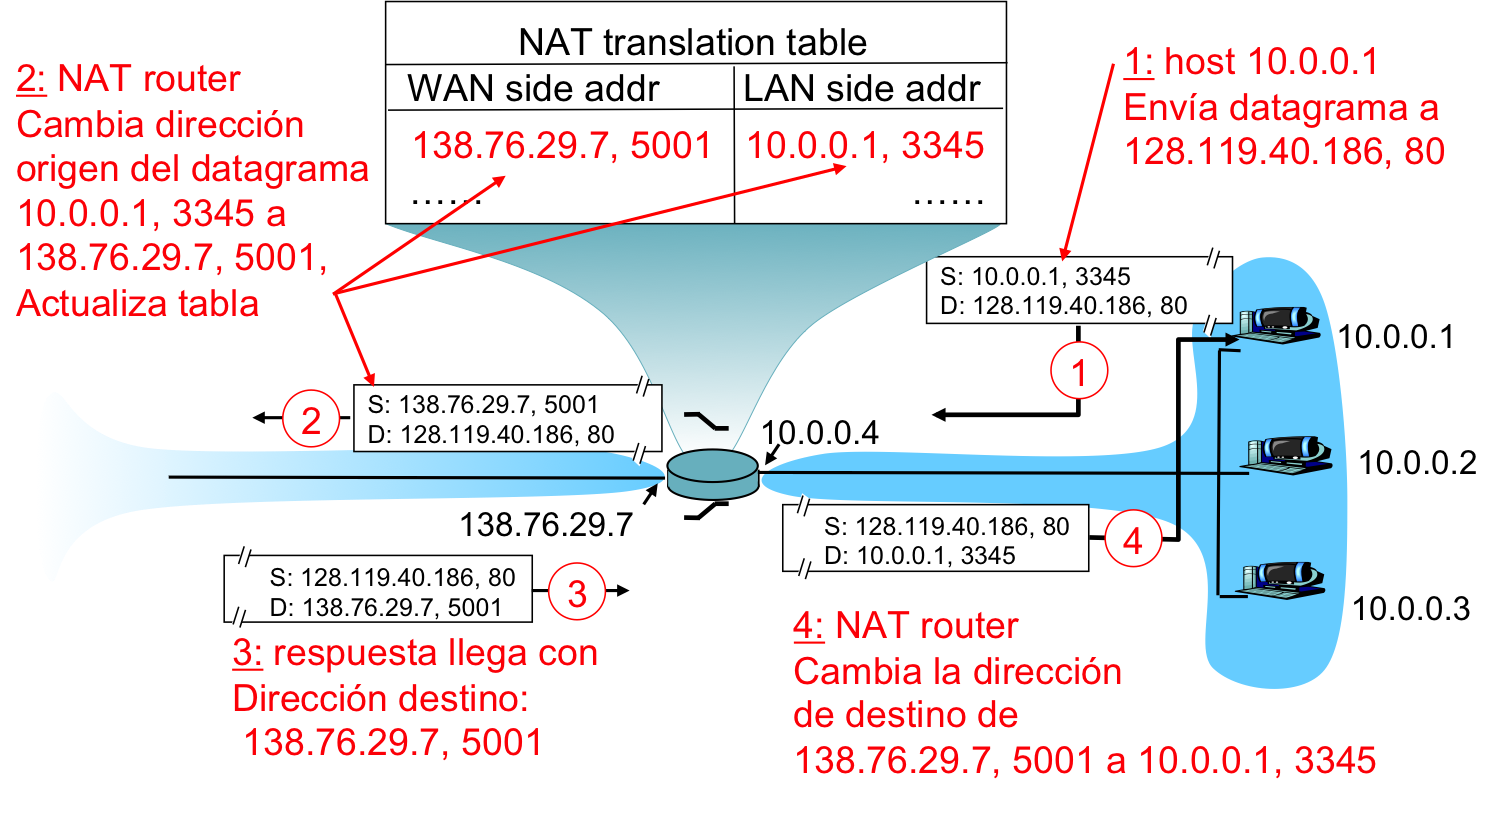
\includegraphics[width=10cm]{figs/07-nat-2.png}
  \end{center}

\end{frame}

%---------------------------------------------------------------------
\begin{frame}
  \frametitle{NAT Traversal}
  \framesubtitle{Solución estática}

   ¿Cómo llegar a un nodo interno?
   \begin{itemize}
     \item Routers deben configurar puertos externos para redirigir a direcciones internas\footnote{Recordar esto al hablar de {\em tunneling}}
     \item Ej: Toda la comunicación a 138.76.29.7:2500 será redirigida a 10.0.0.1:80
   \end{itemize}

  \begin{center}
    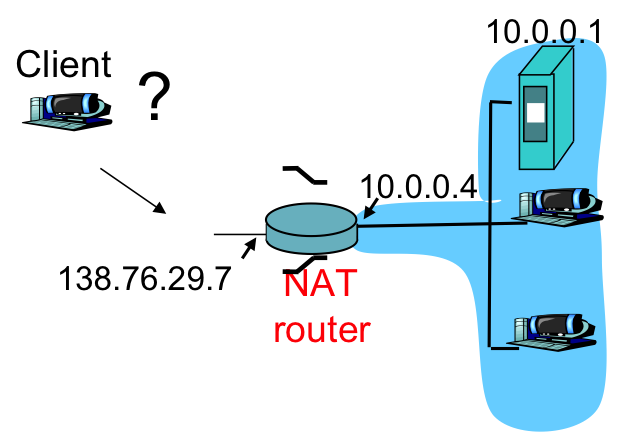
\includegraphics[width=6cm]{figs/07-nat-3.png}
  \end{center}

\end{frame}
%---------------------------------------------------------------------
\begin{frame}
  \frametitle{NAT Traversal}
  \framesubtitle{Solución Plug and Play}
  
  Universal Plug and Play (UPnP), Internet Gateway Device (IGD) protocol
  \begin{itemize}
    \item Permite configurar mapping de puertos a nodos internos dinámicamente
    \item Transparente para el nodo interno
  \end{itemize}
  
\end{frame}


%---------------------------------------------------------------------
\section{ICMP y IPv6}

\subsection{ICMP}
%---------------------------------------------------------------------
\begin{frame}
  \frametitle{ICMP}
  \framesubtitle{Internet Control Message Protocol}
  
  \begin{itemize}
    \item Parte del {\em stack} TCP/IP
    \item Usado para mensajes de diagnóstico y control
    \item Usos principales: {\tt ping}, {\tt traceroute}
    \item Se envían dentro de paquetes IP, pero se tratan de manera especial
  \end{itemize}
  Algunos tipos de mensajes ICMP
  \begin{itemize}
    \item {\tt echo reply} (ping)
    \item {\tt dest. network unreachable}
    \item {\tt dest. host unreachable}
    \item {\tt dest. host unknown}
    \item {\tt echo request} (ping)
    \item {\tt router discovery}
    \item {\tt TTL expired}
    \item {\tt bad IP header}
  \end{itemize}
  
\end{frame}

%---------------------------------------------------------------------
\begin{frame}
  \frametitle{ICMP}
  %\framesubtitle{{\tt ping} y {\tt traceroute}}

  {\tt ping}
  \begin{itemize}
    \item Test de {\em reachability}
    \item {\tt echo request} + {\tt echo reply}
    \item Permite calcular {\em Round Trip Time}
  \end{itemize}
  {\tt traceroute}
  \begin{itemize}
    \item Envía una serie de mensajes {\tt Echo request} con TTL incremental
    \item Cada respuesta {\tt Time Exceeded} permite identificar routers intermedios
    \item Cuando se encuentra el destino, éste devuelve {\tt Echo Reply}
  \end{itemize}

\end{frame}
%---------------------------------------------------------------------
\subsection{IPv6}

\begin{frame}
  \frametitle{IPv6}
  
  Direcciones 128-bit
  \begin{itemize}
    \item $\sim 96\%$ del tráfico aún es IPv4
    \item Formato 8 grupos de 4 dígitos hexadecimales
      \begin{itemize}
        \item {\tt 2001:0db8:85a3:0042:1000:8a2e:0370:7334}
        \item Loopback: {\tt 0000:0000:0000:0000:0000:0000:0000:0001}
        \item Abreviable a: {\tt ::1}
        \item Direcciones IPv4 anotables como: {\tt ::ffff:192.0.2.128}
      \end{itemize}
  \end{itemize}
  
  \begin{center}
    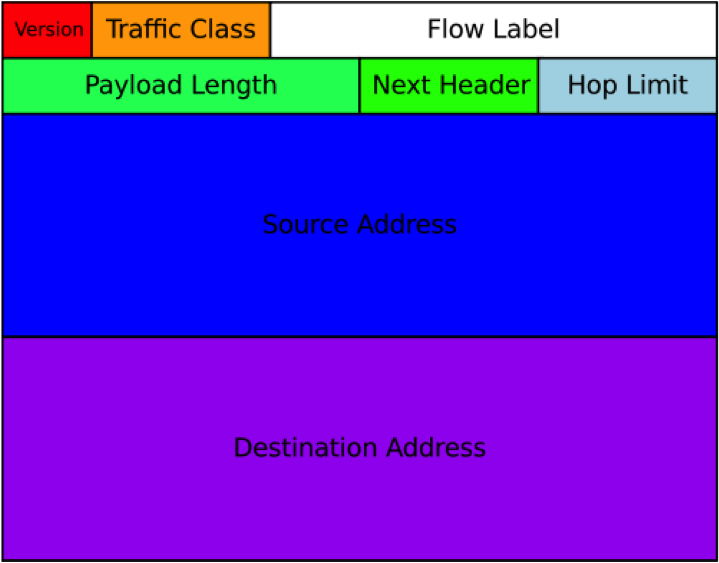
\includegraphics[width=5cm]{figs/07-ipv6.png}
  \end{center}

\end{frame}

%---------------------------------------------------------------------
\begin{frame}
  \frametitle{IPv6}
  \framesubtitle{Transición IPv4 a IPv6}

  Transición no es inmediata
  \begin{itemize}
    \item {\em Dual stack implementation}
    \item {\em Tunneling}
       \begin{itemize}
         \item Tunneling permite utilizar routes IPv4 como intermediarios
    	 \item Paquetes IPv6 se transportan en campo de datos de IPv4
       \end{itemize}
  \end{itemize}
  \begin{center}
    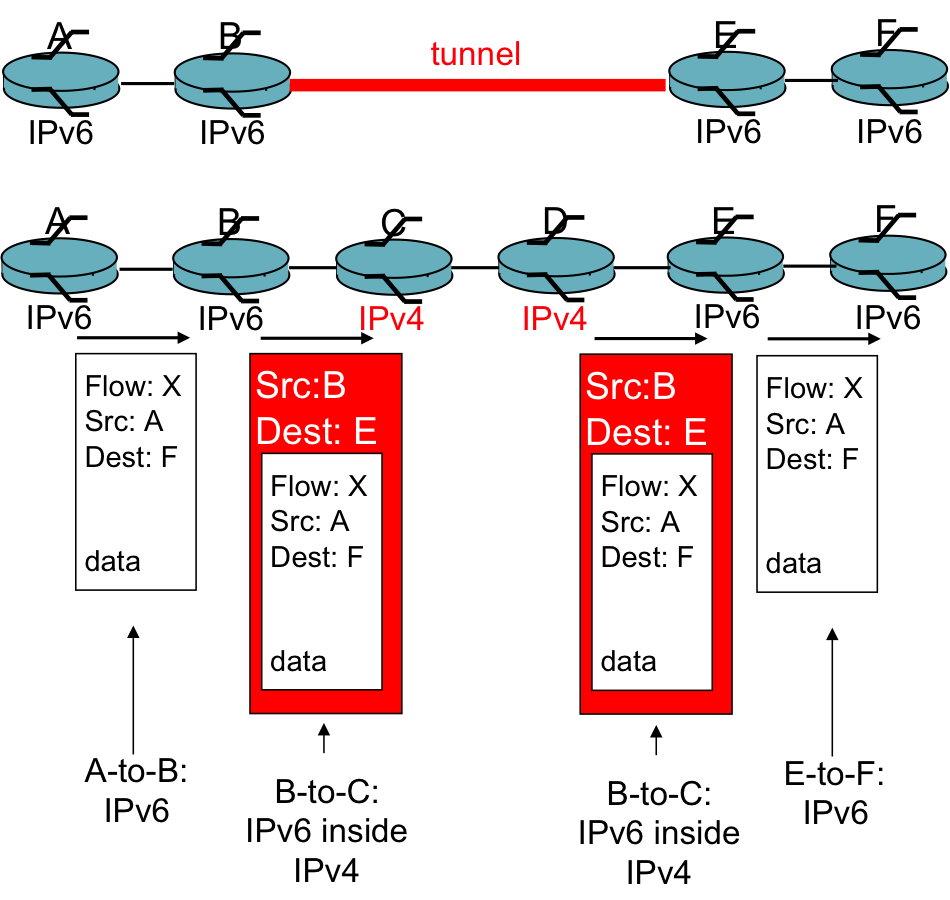
\includegraphics[width=5cm]{figs/07-ipv6-tunnel.png}
  \end{center}

\end{frame}


%---------------------------------------------------------------------
\section{Enrutamiento}

%---------------------------------------------------------------------
\subsection{Algoritmos de Enrutamiento}

\begin{frame}
  \frametitle{Algoritmos de Enrutamiento}

  Objetivo: determinar {\bf el mejor} camino entre {\em router}s para llegar al destino
  \begin{itemize}
    \item Modelado como un grafo, donde cada {\em router} es un nodo y sus conexiones con aristas
    \item ¿Qué significa el mejor camino?
      \begin{itemize}
        \item Depende de la definición de {\em costo} de aristas
        \item Más corto, menos congestionado, mayor ancho de banda, \ldots
      \end{itemize}
  \end{itemize}

  \begin{center}
    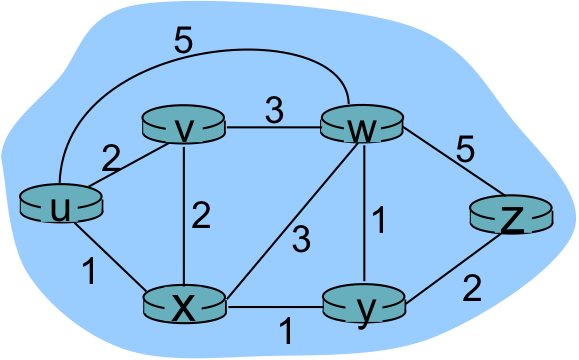
\includegraphics[width=7cm]{figs/07-enrutamiento-grafo.png}
  \end{center}

\end{frame}

%---------------------------------------------------------------------
\begin{frame}
  \frametitle{Tipos de algoritmos}

  Conocimiento de la red
  \begin{itemize}
    \item {\bf Global}. Nodos conocen la topología y costos de enlaces
      \begin{itemize}
        \item Algoritmos que conocen {\em estado del enlace}
      \end{itemize}
    \item {\bf Decentralizados}. Nodos conocen a sus vecinos, y estados de esos enlaces
      \begin{itemize}
        \item Se basan en intercambio de información con vecinos
        \item Algoritmos que conocen {\em vectores de distancia}
      \end{itemize}
  \end{itemize}
  Dinamicidad
  \begin{itemize}
    \item {\bf Estáticos}. Rutas con cambios poco frecuentes
    \item {\bf Dinámicos}. Se actualizan periódicamente en base a costos de enlace
  \end{itemize}
\end{frame}

%---------------------------------------------------------------------
\begin{frame}
  \frametitle{Algoritmos de Estado de Enlace}
  \framesubtitle{{\em Link State} routing}
  
  \begin{itemize}
    \item Cada nodo envía su información de conectividad a sus vecinos
    \item Información se comunica a los demás vía {\em flooding}
    \item Cuando todos tiene información de la topología, cada uno calcula las rutas más cortas
      \begin{itemize}
        \item Algoritmo de Dijkstra (1957)
      \end{itemize}
  \end{itemize}
  
  \begin{center}
    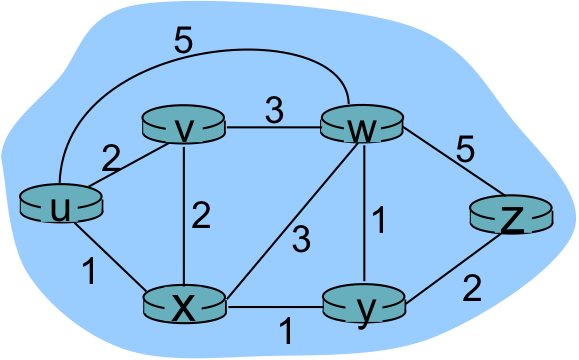
\includegraphics[width=5cm]{figs/07-enrutamiento-grafo.png}
  \end{center}

  
\end{frame}

%---------------------------------------------------------------------
\begin{frame}
  \frametitle{{\em Link State} routing}
  \framesubtitle{Algoritmo de Dijkstra}

  \begin{center}
    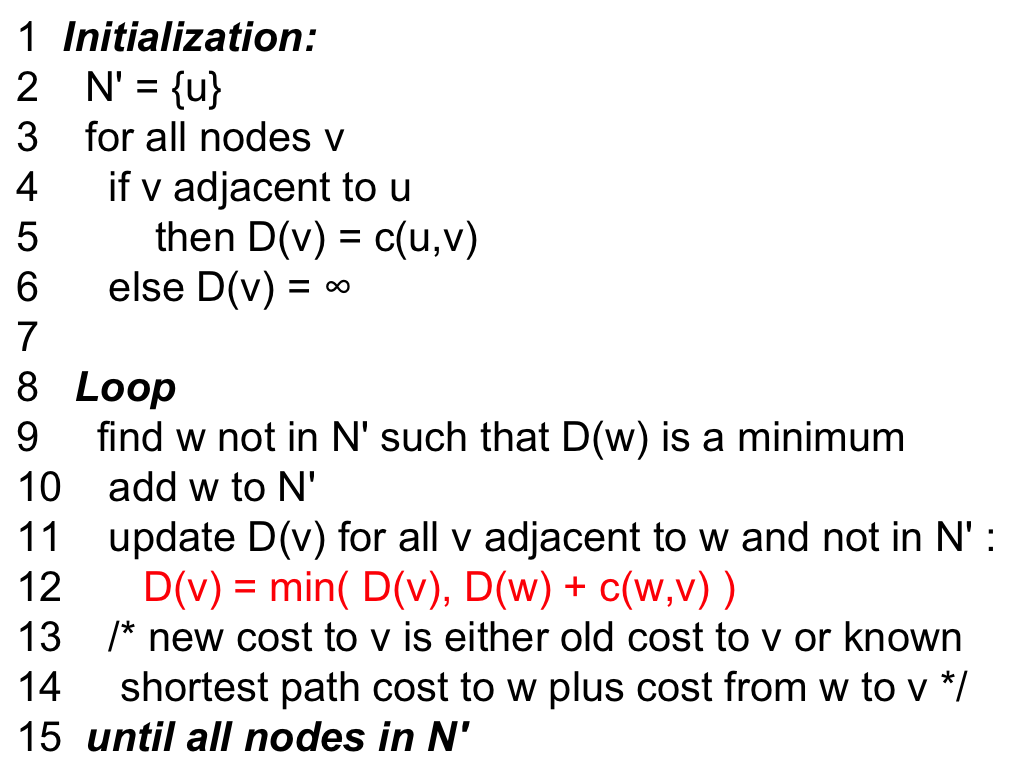
\includegraphics[width=9cm]{figs/07-ls-dijkstra.png}
  \end{center}

\end{frame}

%---------------------------------------------------------------------
\begin{frame}
  \frametitle{{\em Link State} routing}

  Rutas más cortas desde {\em u}
  \begin{center}
    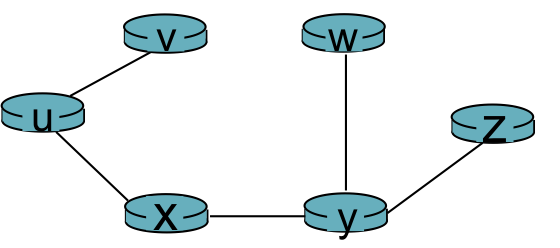
\includegraphics[width=5cm]{figs/07-ls-u.png}
  \end{center}
  Tabla de ruteo de {\em u}
  \begin{center}
    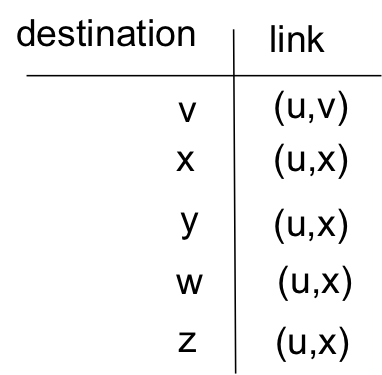
\includegraphics[width=4cm]{figs/07-ls-route.png}
  \end{center}

\end{frame}


%---------------------------------------------------------------------
\begin{frame}
  \frametitle{Algoritmo de Vectores de Distancia}

  Basado en ecuación de Bellman-Ford
  \[
    d(x,y) = min_v\{c(x,v) + d(v,y)\}
  \]
  \begin{itemize}
    \item Cada nodo mantiene una tabla de la mejor ruta a sus vecinos
    \item Cada nodo comparte su tabla con sus vecinos
    \item Cuando la información se ha propagado a todos los nodos, cada uno conoce las mejores rutas
    \item Diferencia con LS: se propaga información de rutas, en lugar de enlaces
  \end{itemize}
  Funciona de manera distribuida
  \begin{itemize}
    \item Se gatilla ante cambios locales de costos
    \item Se gatilla al recibir mensajes de vecinos
  \end{itemize}

\end{frame}
%---------------------------------------------------------------------
\begin{frame}
  \frametitle{Algoritmo de Vectores de Distancia}

  \begin{center}
    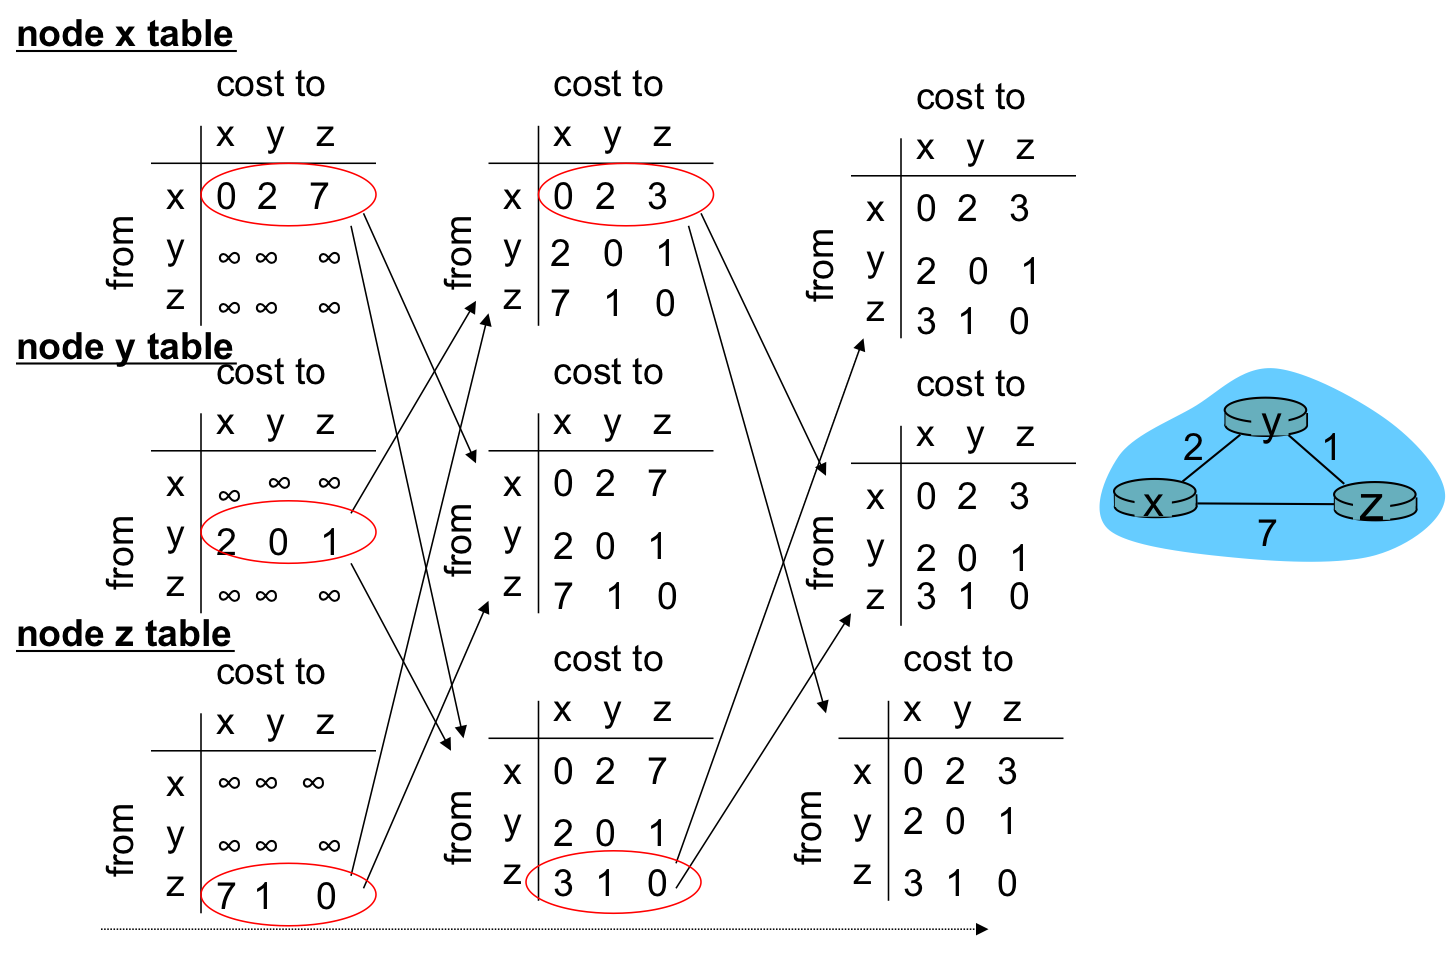
\includegraphics[width=10cm]{figs/07-dv.png}
  \end{center}

  
\end{frame}
%---------------------------------------------------------------------
\begin{frame}
  \frametitle{Algoritmo de Vectores de Distancia}
  \framesubtitle{Count-to-Infinity}
  
  \begin{itemize}
    \item Las noticias buenas se propagan rápido
    \item Noticias malas pueden generar conteos infinitos
  \end{itemize}

  \begin{center}
    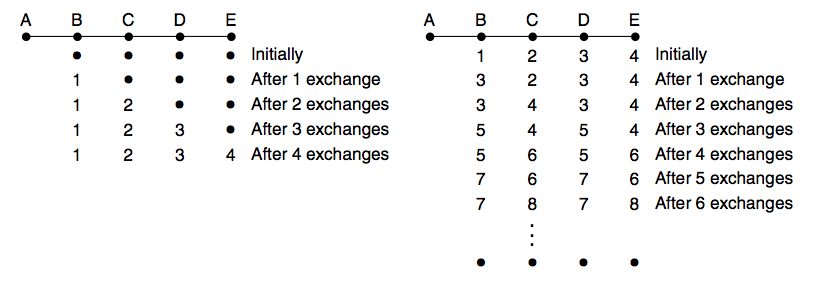
\includegraphics[width=10cm]{figs/07-dv-infinity.png}
  \end{center}

\end{frame}
%---------------------------------------------------------------------
\begin{frame}
  \frametitle{Link State vs Distance Vector}
  
  Link State
  \begin{itemize}
    \item $N$ nodos, $E$ enlaces: $O(NE)$ mensajes
    \item Ante errores, se propaga ausencia de enlace
  \end{itemize}
  Distance Vector
  \begin{itemize}
    \item Tiempo de convergencia indeterminado
    \item Ante errores, se propaga el error. Puede generar ciclos infinitos.
  \end{itemize}
  
\end{frame}
%---------------------------------------------------------------------
\subsection{Enrutamiento de Internet}

\begin{frame}
  \frametitle{Enrutamiento interno y externo}
  
  No es factible almacenar tablas para todos los routers de Internet
  \begin{itemize}
    \item Internet se compone de {\em Sistemas Autónomos} (AS) interconectados
    \item Algoritmos intra-AS resuelven ruteo en un subconjunto de la red
    \item Algoritmos inter-AS ayudan a determinar {\em forwading tables} entre distintos AS
  \end{itemize}
\end{frame}
%---------------------------------------------------------------------
\begin{frame}
  \frametitle{IGP: Interior Gateway Protocols}

  Enrutamiento intra-AS
  \begin{itemize}
    \item RIP: Routing Information Protocol
    \item OSPF: Open Shortest-Path First
    \item IGRP: Interior Gateway Routing Protocol (CISCO Propietary)
  \end{itemize}

\end{frame}
%---------------------------------------------------------------------
\begin{frame}
  \frametitle{RIP: Routing Information Protocol}

  Algoritmo de vector de distancias
  \begin{itemize}
    \item Uno de los más antiguos (implementado en ARPANet)
    \item Métrica: número de saltos ({\em hops})
    \item Envía actualizaciones cada 30 segundos
    \item Mecanismos para evitar errores
      \begin{itemize}
        \item Split Horizon: Evita propagación de rutas redundantes
        \item Poison reverse: Limita la cantidad de saltos. Más de 15 saltos se considera $\infty$
        \item Holddown: Evita actualizar rutas por un tiempo antes un aviso de {\em network unreachable}
      \end{itemize}
  \end{itemize}

\end{frame}

%---------------------------------------------------------------------
\begin{frame}
  \frametitle{OSPF: Open Shortest-Path First}

  Algoritmo del tipo {\em Link-State}
  \begin{itemize}
    \item Muy similar a IS-IS (Interior System - Interior System)
    \item Anuncios transportados directamento en encabezados IP
    \item Permite propagar múltiples rutas con métricas para diferentes
          tipos de medios
    \item Permite implementaciones jerárquicas
  \end{itemize}

  \begin{center}
    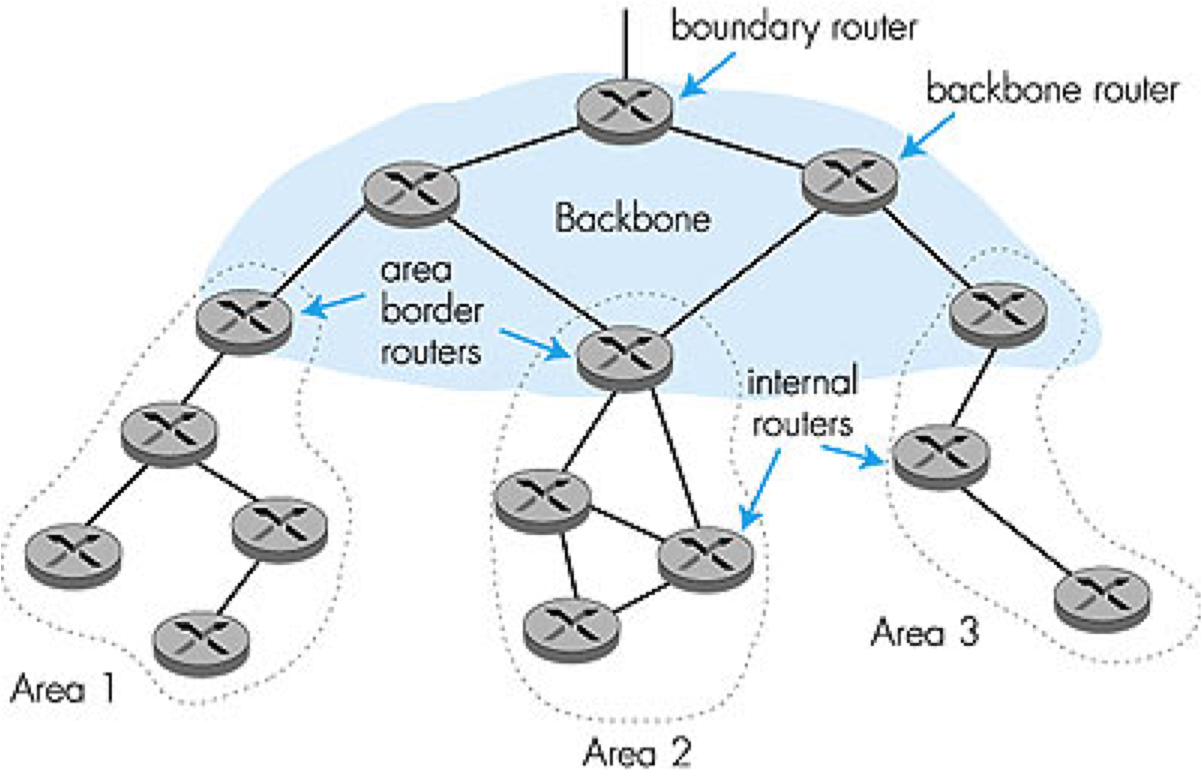
\includegraphics[width=6cm]{figs/07-ospf-jerarquico.png}
  \end{center}

\end{frame}
%---------------------------------------------------------------------
\begin{frame}
  \frametitle{BGP: Border Gateway Protocol}

  Estándar de facto para comunicación Inter-AS
  \begin{itemize}
    \item Permite conectar una subred anunciar su existencia a Internet
    \item Provee medios para:
      \begin{itemize}
        \item Obtener información de {\em reachability} de otras subredes
        \item Propagar información de {\em reachability} a nodos internos
        \item Determinar buenas rutas o otras subredes
      \end{itemize}
    \item Parejas de routers (pares BGP) intercambian información de ruteo
      \begin{itemize}
        \item Sesiones TCP semipermanentes (port 179)
      \end{itemize}
  \end{itemize}
\end{frame}

%---------------------------------------------------------------------
\begin{frame}
  \frametitle{BGP: Border Gateway Protocol}

  Información se propaga a través de {\em prefijos de reachability}
  \begin{itemize}
    \item Nodos guardan información de {\em reachability} en su tabla de reenvío
    \item Decisión se toma en basa a {\em reachability} y otros atributos
  \end{itemize}
  \begin{center}
    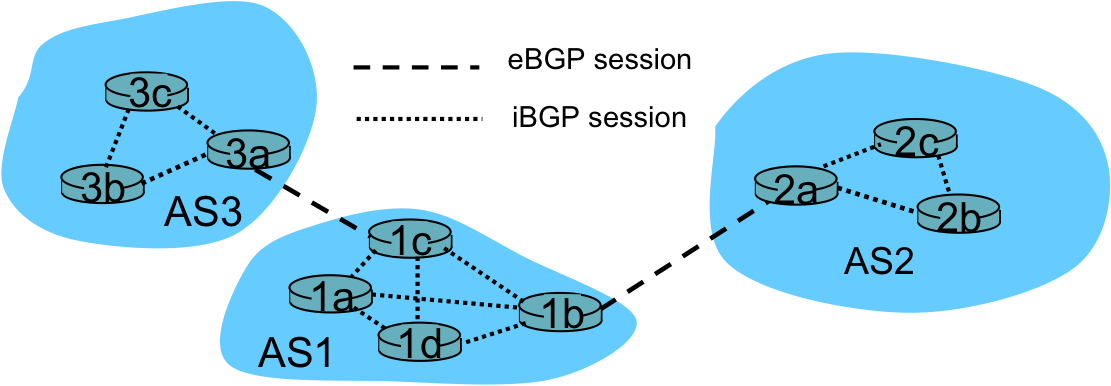
\includegraphics[width=8cm]{figs/07-bgp.png}
  \end{center}

\end{frame}
%---------------------------------------------------------------------
\begin{frame}
  \frametitle{BGP: Border Gateway Protocol}

  \begin{itemize}
    \item AS-PATH: ASs por los que ha pasado el prefijo
    \item NEXT-HOP: Router de destino del anuncio
  \end{itemize}

  \begin{center}
    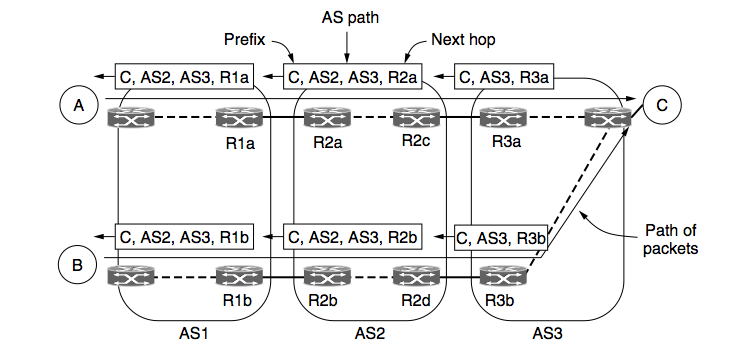
\includegraphics[width=10cm]{figs/07-bgp-2.png}
  \end{center}


\end{frame}

%---------------------------------------------------------------------
\begin{frame}
  \frametitle{BGP: Border Gateway Protocol}

  Routers pueden decidir aceptar o rechazar los anuncios de rutas
  
  Selección de rutas puede tomar múltiples criterios
  \begin{itemize}
    \item Decisión política
    \item AS-PATH más corto
    \item Router NEXT-HOP más cercano
  \end{itemize}

\end{frame}
%---------------------------------------------------------------------
\begin{frame}
  \frametitle{BGP: Border Gateway Protocol}

  \begin{center}
    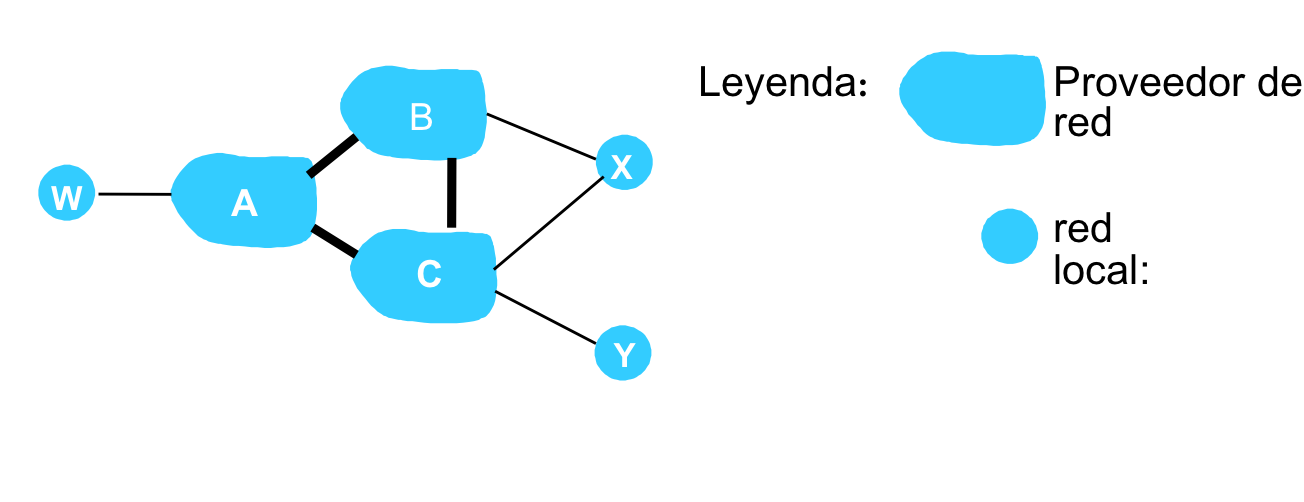
\includegraphics[width=10cm]{figs/07-bgp-rutas.png}
  \end{center}

  ISPs: A,B,C; Clientes: X,W,Y
  \begin{itemize}
    \item $A$ anuncia a $B$ el camino $(A,W)$
    \item $B$ anuncia a $X$ el camino $(B,A,W)$
    \item ¿Debería $B$ anunciar a $C$ el camino $(B,A,W)$?
      \begin{itemize}
        \item $B$ no obtiene beneficio por enrutar $(C,B,A,W)$
        \item $B$ quiere enrutar sólo a sus clientes
        \item $B$ quiere forzar a que $C$ deba enrutar hasta $W$ a través de $A$
      \end{itemize}
  \end{itemize}

\end{frame}

%---------------------------------------------------------------------
\end{document}